\setcounter{chapter}{2}
\setchapterabstract{This chapter explores EU merger control, focusing on the legal framework established by Regulation 139/2004. It outlines the definition of concentration, where a lasting change in control leads to structural market changes, and the rationale for merger review, which aims to prevent anti-competitive effects while acknowledging potential efficiencies or reallocation benefits. Mergers are less stringently regulated than cartels due to their long-term nature and potential pro-competitive effects. The notification process requires pre-approval for mergers exceeding turnover thresholds, ensuring compliance through fines and dissolution for violations. Horizontal mergers are scrutinized for market dominance, while vertical and conglomerate mergers are assessed for access and foreclosure risks. Jurisdictional issues emphasize the one-stop-shop principle, granting the EU Commission exclusive authority for cases with Community dimensions, while Member States can intervene for legitimate non-competition interests, such as security or media plurality. Remedies, including divestitures, aim to balance competition and private interests.}
\chapter{Mergers and Acquisitions \\ Concentrations}
\vspace{-1.5cm}

\setcounter{chapter}{13}
{\chaptoc\noindent\begin{minipage}[inner sep=0,outer sep=0]{0.9\linewidth}\section*{Main Legal Sources - European Level}\end{minipage}}

\begin{itemize}
    \item \textbf{Reg. 139/2004:} Notion of concentration, Notification, Stand-still obligation, Referral to/from Member States, Standard of appraisal, Decisional powers, Remedies, Fines in case of “gun jumping” and other violations

    \item \textbf{Jurisdictional Notice:}
    \begin{itemize}
        \item Notion of concentration
        \item Sole/joint control
        \item Notion of undertaking
        \item Turnover
        \item Joint ventures
    \end{itemize}
    \item \textbf{Notices on:}
    \begin{itemize}
        \item Horizontal mergers (how to evaluate horizontal mergers)
        \item Non-horizontal mergers (vertical and conglomerate mergers)
    \end{itemize}
    \item \textbf{Notice on remedies:} To avoid any perverse effect while allowing the parties to merge.
    \item \textbf{Other regulations and notices:} Procedures, timing, forms, Simplified notification, Best practices, Ancillary restrictions
\end{itemize}

\newpage
\section{Notion of Concentration}

    \Definition{
    Some authors describe concentrations as a process that, by decreasing the number of independent firms on the market, determines an increase in the degree of concentration on that market.
    }{Concentration}

    The aforementioned description has the advantage of representing the possible economic outcome of a (horizontal) concentration between two independent firms on the same relevant market. The number of firms decreases and, accordingly, there is an increase of the acquiring party’s market power, and as a consequence an increase in the degree of concentration characterizing that relevant market.

    \noindent
    However, the previous description (\( \downarrow \# \text{ players} \rightarrow \uparrow \text{concentration} \)) is (partially) wrong!

    \begin{enumerate}[label=\alph*.]
        \item A structural concentrative effect can be obtained even if the total number of economic agents does not decrease.
        
            It is even possible to obtain a structural concentrative effect notwithstanding an increase in the total number of independent undertakings.
            
            \Example{For example, if Stellantis and Volvo form a joint venture to which they confer all their trucks business, the total number of firms increases (Stellantis, Volvo, and the JV), together with an increase in the degree of concentration (in the market for trucks).}

        \item The effect on the degree of market concentration is linked to the prior competitive relationship between the merging parties. If Stellantis acquires Oxford University Press, there is no (direct) effect on the car market level of concentration (and similarly no effect on the academic publishing market).
    \end{enumerate}

        \subsubsection*{Alternative definition of merger}

            \Definition{A concentration is a change of control (ownership, possession, right to use) on a lasting basis of the assets/business of one or more undertakings.}{Concentration - Alternative Definition}

            Only a lasting change in the control of (the assets of) the undertakings concerned can in fact bring about a lasting change in the structure of the market. “Concentrations” can be thought of as the result of a process according to which one undertaking may strengthen its position on the market (not by internal growth but) by drawing (acquiring, absorbing) from third parties assets (external growth).\sn{\Note{There are many other different ways through which it is possible to obtain the economic effect of a concentration, e.g. by forming a joint venture but also through divisions and/or demergers of existing undertakings!}}

            \Example{ 
            \textbf{A merger}: the new entity will absorb all the assets of both the merging parties or, for mergers by acquisition, the surviving party will acquire all the assets of the merged party.
            FCA and Peugeot merge into a new entity (Stellantis). Stellantis inherits all the assets previously belonging to FCA and Peugeot.}
            
            \Example{The acquisition of all (or parts of) the assets (or business units) of another undertaking is a concentration. FCA acquires all the business assets of Peugeot (or... the truck business)}

            \Example{The acquisition of all (or parts of) the assets (or business units) of another undertaking is a concentration. FCA acquires all the business assets of Peugeot (or... the truck business)}

\section{The Merger Paradox}

    \noindent
    Compare a “cartel” and a “merger” between A and B. At first glance, a merger should be treated more harshly than a cartel. In fact:

        \begin{itemize}
            \item \textbf{Cartel:} 
            \begin{itemize}
                \item Has the object of restricting competition within the parties (price fixing, market sharing, etc.).
                \item Is “unstable” and “breakable” (it can be terminated by the parties, by external competition, etc.).
                \item \textbf{Temporary} in nature.
            \end{itemize}
            \item \textbf{Merger:}
            \begin{itemize}
                \item Eliminates any kind of competition between the parties.
                \item Basically permanent in nature with \textbf{lasting effects}.
            \end{itemize}
        \end{itemize}
        
        \noindent
        At first glance, a temporary reduction in competition is better than a permanent elimination of any competitive stimulus between the parties.
        
        \noindent
        \textbf{However, and quite paradoxically, mergers are treated less harshly and in any case more flexibly than cartels.}
        
        \Example{
        A naked agreement between A and B would likely be prohibited even with a very low combined market share (it’s a \textbf{by object restriction}). \\
        A merger between the same parties would likely be approved even with quite large market shares (e.g., 30\%). \\
        \begin{itemize}
            \item Cartel A + B: \textbf{Rejected/Sanctioned} \\
            \item Merger A + B: \textbf{Approved}
        \end{itemize}
        }

\newpage

    \subsection{Rationale}

        \begin{enumerate}
            \item \textbf{First,} mergers may bring along efficiencies by developing new products or by reducing production or distribution costs.
            \begin{itemize}
                \item In practice, it is quite difficult to prove efficiencies; several economic studies show that, \textit{ex post}, mergers are not efficiency-enhancing. 
                \item See Kwoka, \textit{Mergers, Merger Control, and Remedies}, MIT Press, 2014.
                \item Mergers may produce efficiencies especially when the merging parts are relatively small (i.e., the \textit{ex post} market share is still relatively small).
            \end{itemize}
            \item \textbf{Second,} mergers may help the fundamental function of reallocating entrepreneurial capabilities. 
            \begin{itemize}
                \item Consider some of the many reasons why the owner of a firm might wish to sell its property:
                \begin{enumerate}[label=(\alph*)]
                    \item Lack of financial resources.
                    \item Tiredness or ineptitude.
                    \item Desire to invest in new and innovative markets.
                \end{enumerate}
                \item Prohibiting M\&A could result in firms remaining in the hands of entrepreneurs who no longer want or are unable to manage them, or who could achieve better results in other fields.
                \item This theory suggests we should favour transfers of business, i.e., wealth flows.
                \item \textbf{However,} this does not mean we should favour the transfer of such business to a particular firm if that transfer leads to excessive market power.
            \end{itemize}
            \item \textbf{Third,} by combining two or more firms, mergers entail structural effects that are, by definition, long-lasting and basically irreversible.
            \begin{itemize}
                \item Therefore:
                \begin{enumerate}[label=(\alph*)]
                    \item It is very difficult to restore competition fully once a merger takes place and produces its effects on the structure of the market.
                    \item Furthermore, any attempt to re-establish competition after the fact is usually very costly for the parties and all their stakeholders (employees, customers, creditors, etc.).
                \end{enumerate}
            \end{itemize}
            \Remark{
            This is the reason why a mandatory pre-merger notification procedure is usually in force: e.g.: EU Reg. 139/2004.
            }
            This obviously does not explain directly why a merger should be treated better than a cartel between the same parties!
            However, the fact that antitrust authorities must adopt an ex-ante analysis, focused on possible future, foreseeable, but still uncertain effects deriving from mergers suggests a more cautious, reasonable, and open evaluation of all the possible constraints and reactions to an hypothetical increase in market power.
        \end{enumerate}   

\newpage

        \begin{enumerate}
        \setcounter{enumi}{3}
            \item \textbf{Fourth,} some (old-Chicago school) economists argue that what is really important is to avoid chilling pro-competitive mergers and innovation. Being lenient with mergers is considered a minor mistake because:
            \begin{enumerate}[label=(\alph*)]
                \item Markets tend to self-correct, at least in the long run.
                \item The task of government and authorities is to keep market entry open and easy (contestable markets).
                \item Antitrust authorities may still use their enforcement powers to limit the actions of dominant firms.
            \end{enumerate}
            \textbf{This suggestion proved to be quite dangerous!}
            \begin{itemize}
                \item Between 1990 and 2020, especially in the US, there was a decrease in merger enforcement by the Antitrust Division and FTC (e.g., in pharma, telecoms, hi-tech, internet, distribution outlets, and services).
                \item This lenient approach contributed to:
                \begin{itemize}
                    \item A substantial increase in market concentration.
                    \item An increase in prices and margins earned by many “big players.”
                    \item A decrease in salaries, investment, productivity, and growth.
                \end{itemize}
            \end{itemize}
        \end{enumerate}

        \Remark{
            Philippon started with a mundane question:
                \begin{quote}
                    “Why on earth are US cell phone plans so expensive? Or, to broaden it a little further, why do consumers in Europe or Asia pay less for cellular service and, on average, get much more?”
                \end{quote}
                His answer: Lack of competition, combined with lobbying and campaign contributions by many “big players” that have weakened antitrust regulators.}

            Zingales, Posner \& Lancieri tell the same story\sn{\Note{In the last years, we have witnessed the rise of many opponents to the Chicago’s mainstream view, but they are either too radical or have a “confused” view about which goals antitrust should pursue and how}}. All the decision-makers involved (the US Supreme Court, judges, the agencies, many politicians, and the government) are or became in fact pro-business, because of lobbying, common interests, economic links, etc.             

        \subsubsection{Recent Changes}

            \textbf{In the U.S.:} Under the leadership of Lina Khan, tougher merger enforcement and new, stricter horizontal merger guidelines.
            However, rumors suggest that the new Trump administration may repeal these guidelines within the first 100 days. \\

            \noindent
            \textbf{In Europe:} Tougher enforcement and new theories of harm, particularly in the area of digital ecosystems.

            \noindent
            However, we have mixed signals: Draghi report and new Commissioner Ribera mandate emphasize:
                \begin{enumerate}
                    \item Support for competition.
                    \item The need for stronger firms capable of competing at a global level.
                    \item The level of private investment required to be innovative and maintain a position at the forefront of technological advancement is incompatible with the average small size of European firms.
                \end{enumerate}

        \subsubsection{Consumer Surplus' Role in Merger Analysis}

            \noindent
            \(\Rightarrow\) \textbf{TS? (Chicago)} \\
            \(\Rightarrow\) \textbf{CS? (CS’s 5 stars?). Motta: Tougher enforcement?} \\
            
            \noindent
            \textbf{“New Brandeis” scholars:}
            \begin{itemize}
                \item Effects on employment: Should we forbid a merger that induces some efficiencies but simultaneously results in wage cuts and layoffs for many workers?
                \item Sustainability and environment.
                \item Small business: Amazon has already eliminated many bookstores and is now over-exploiting small sellers who are \textit{“obliged”} to use its platform.
                \item Democracy: Economic power, lobbying, etc.
                \item Privacy: The Facebook/WhatsApp merger enables better extraction of personal data, which can then be used to influence our choices and (political) behavior.
            \end{itemize}
            
            \noindent
            Economic power should not interfere with political power and threaten the stability of a democratic regime. Thus, a wider standard of evaluation should be adopted.

            \Remark{Dealing with mergers its not only dealing with economic forecasting models. It’s also a complex legal/policy issue. Furthermore, sometimes firms have to deal with antitrust jurisdictions where goals (explicit or hidden) are very different from total surplus, consumer surplus, competitive structure of the market, etc. Merger policy may sometimes be guided by industrial policy goals or even nationalistic/populistic goals.}

            \noindent
            For lawyers, mergers may become a (well-paid) nightmare!!!
            
            \begin{enumerate}
                \item Some mergers between global players must be notified to 50–60 jurisdictions around the world, with no harmonization on:
                \begin{itemize}
                    \item Procedural rules (notion of concentration, mandatory filing, stand-still obligation, timing, fees, etc.).
                    \item Substantive evaluation (dominance, lessening of competition, etc.).
                \end{itemize}
                \item Consequences of procedural and/or substantive breaches can be very serious:
                \begin{itemize}
                    \item Heavy fines.
                    \item Demerger or divestiture orders.
                \end{itemize}
                \item In some jurisdictions, the pressure and powers of governments to allow/block mergers may be very strong (e.g., Siemens-Alstom).
            \end{enumerate}

\newpage
\section{Merger Notification}

    \noindent
    \subsubsection*{Rule}
    
    \begin{itemize}
        \item In the EU, we have a system of:
        \begin{enumerate}[label=\alph*.]
            \item Mandatory,
            \item Ex-ante notification of,
            \item Concentrations (better: concentration proposals),
            \item When they exceed certain thresholds in terms of turnover.
        \end{enumerate}
        \item The Commission analyzes the likely effects of the combination \textbf{before} the proposed merger takes place. During this time, a stand-still obligation applies.
        \begin{itemize}
            \item If the outcome of the appraisal process is \textbf{positive}, the merger is allowed to proceed.
            \item If the outcome is \textbf{negative}, the parties must refrain from proceeding with the merger or propose remedies to address the competitive concerns identified by the Commission.
        \end{itemize}
    \end{itemize}
    
    \subsubsection*{Exception}
    
    \begin{itemize}
        \item Since 2022, \textit{Art. 22 referrals} allow Member States and/or third parties to refer under-threshold mergers if certain conditions are met.
        \item In such cases, the appraisal may also occur \textbf{ex post}.
    \end{itemize}

    \subsection{Thresholds}

    When designing EU notification thresholds, various potentially conflicting elements had to be considered:
    
    \begin{itemize}
        \item \textbf{SOME OR ALL?} Should we require any merger to undergo prior mandatory notification? This is impractical and too costly. Therefore, only the large and potentially relevant ones are targeted.
        \item \textbf{EU vs. MS?} Member States (MS) are protective of their national merger jurisdiction. The power to clear or block a merger is still considered an important, albeit ambiguous, tool of economic and industrial policy (and protectionism). This raises tensions between domestic and EU levels.
        \item \textbf{EFFICIENCY AND LEGAL CERTAINTY.} Firms strongly prefer a “one-stop-shop system” for merger notification. If the European thresholds are exceeded:
        \begin{itemize}
            \item The Commission should have sole jurisdiction to make decisions under the Merger Regulation.
            \item No Member State should apply its national competition laws to concentrations with a Community dimension.
        \end{itemize}
    \end{itemize}

\newpage
    \noindent
    \textbf{A concentration has a Community dimension where:}
    \begin{enumerate}[label=\alph*)]
        \item The combined aggregate worldwide turnover of all the undertakings concerned exceeds €5,000 million; and
        \item The aggregate Community-wide turnover of each of at least two of the undertakings concerned exceeds €250 million; 
        \item \textbf{Unless} each of the undertakings concerned achieves more than two-thirds of its aggregate Community-wide turnover within one and the same MS.
    \end{enumerate}
    
    \noindent
    A concentration not meeting the above thresholds has a Community dimension where:
    \begin{enumerate}[label=\alph*)]
        \item The combined aggregate worldwide turnover of all the undertakings concerned exceeds €2,500 million;
        \item In each of at least 3 MS, the combined aggregate turnover of all the undertakings concerned exceeds €100 million;
        \item In each of at least 3 MS included for point (b), the aggregate turnover of each of at least 2 of the undertakings concerned exceeds €25 million;
        \item The aggregate Community-wide turnover of each of at least 2 of the undertakings concerned exceeds €100 million;
        \item \textbf{Unless} each of the undertakings concerned achieves more than two-thirds of its aggregate Community-wide turnover within one and the same MS.
    \end{enumerate}

    \subsubsection{Turnover as a Universal Solution}

        \begin{itemize}
            \item Turnover depends on the characteristics of the market. For example, the most important Italian law firm has a turnover approximately equal to that of a local oil company that owns 10 highway service stations.
        
            \item In some industries, some firms offer their goods for free (at least in a start-up phase, at very low prices, or even at zero prices). 

            \Example{For example, when Facebook acquired WhatsApp, its turnover was negligible and is now zero. Until very recently, Waze, Zoom, Instagram, and many other significant tech players had zero turnover as well.}
        
            \item Firms willing to maintain their monopoly can pay to incorporate and/or kill potential competitors still not on the market (e.g., start-ups).
            
            \Example{Examples include Google Maps/Waze, Facebook/Instagram, Zomato/UberEats. Between 2020 and 2020, GAMAF conducted more than 1,000 acquisitions, most of which were not scrutinized.}

        \end{itemize}
        

\newpage
        \subsubsection*{Is turnover always the best solution?}
        
        Not always, we can also introduce transaction value (but not market shares).

        \begin{itemize}
            \item Modifying laws and regulations is very difficult and burdensome, especially in this period of renewed populism and nationalism.
            \begin{itemize}
                \item If you want to change a regulation, you must obtain consensus from Member States (MS).
                \item Such a change would entail a reduction in MS jurisdiction (i.e., power to monitor/decide) in favour of the Commission.
            \end{itemize}
        
            \item The Commission found an alternative solution: Article 22 of Regulation 139/2004. A Member State may ask the Commission to investigate a merger that does not meet the EU threshold if:
            \begin{enumerate}
                \item it may influence trade between Member States; and
                \item it risks significantly affecting competition at the EU level.
            \end{enumerate}
            
            \item As per the current interpretation of the law (2024 EU Court of Justice, Illumina case):
            \begin{itemize}
                \item Member States can exercise this power only if the merger satisfies at least the threshold provided at the national level.
                \item However, in some countries, these thresholds are extremely low.
            \end{itemize}
        \end{itemize}

        \subsubsection*{The EU Procedure}

            \begin{figure}[ht]
                \centering
                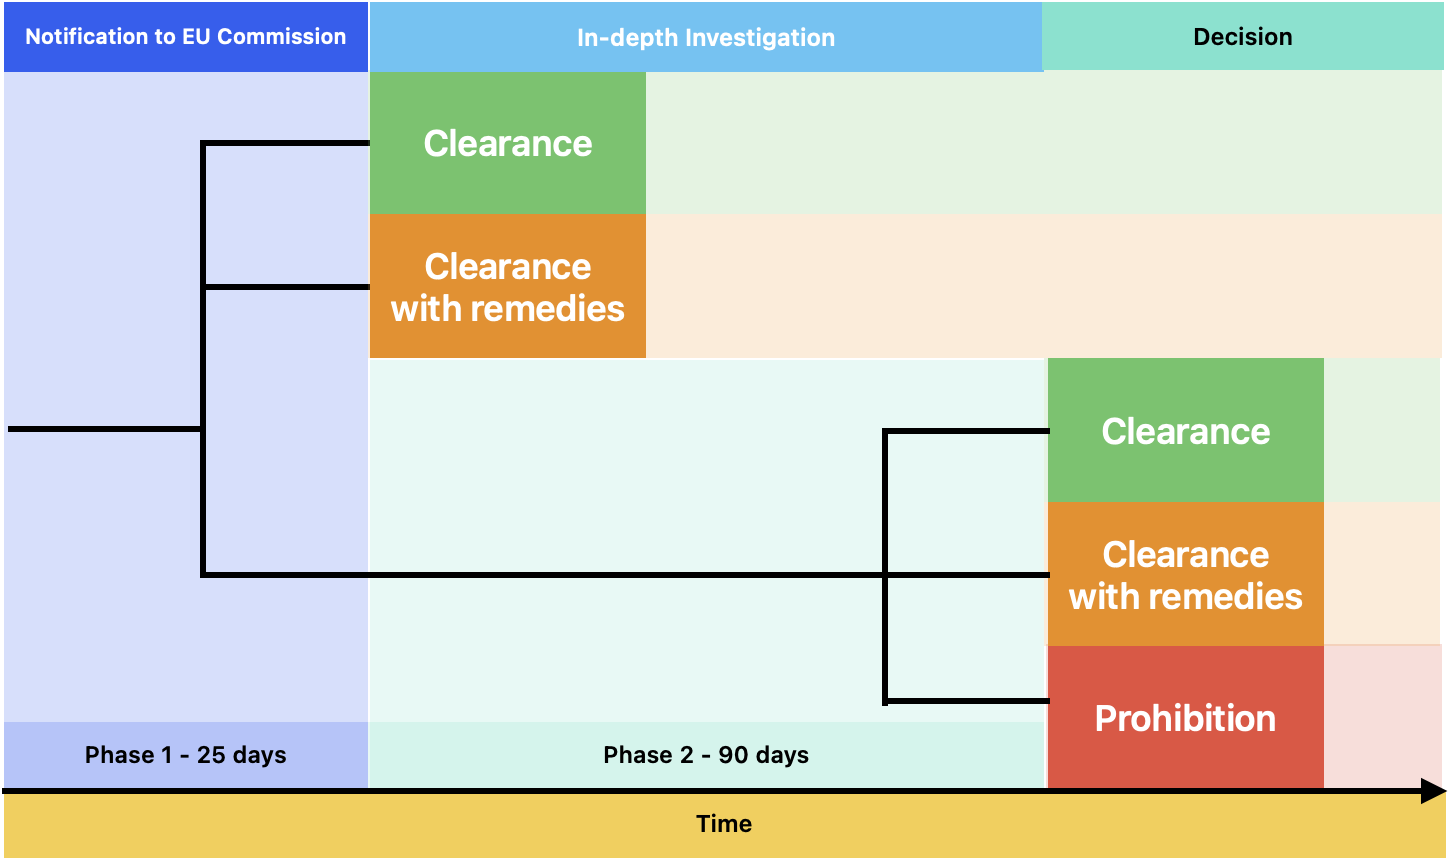
\includegraphics[width=1\linewidth]{graphics/L13-1.png}
            \end{figure}


\newpage
\section{Merger Appraisal}

    \begin{itemize}
        \item In \textbf{phase one}, the Commission scrutinizes jurisdiction (whether the notified operation qualifies as a merger/concentration according to the law; if it meets the quantitative thresholds that trigger mandatory prior notification); decides whether to accept or propose a referral to a Member State; and clears the concentration if no anticompetitive effects are foreseen (no smell of burning).
    
        \item In \textbf{phase two}, initiated only if there are serious risks of harmful effects, the Commission conducts an in-depth market investigation using its investigative powers (e.g., requests for information, inspections, copies of documents, asking for explanations on facts or documents, and recording responses). In Europe, parties have strong rights of defense, including the right to access the file, the right to be heard, and the right to submit studies and observations in writing, including those from their experts.
    \end{itemize}

    \Remark{Article 3(2) of Regulation 139/2004 forbids concentrations which would significantly impede effective competition, in the common market or in a substantial part of it, in particular as a result of the creation or strengthening of a dominant position.}

    In the US the test is slightly different: Section 7, Clayton Act prohibits mergers and acquisitions when the effect may be to substantially lessen competition, or to tend to create a monopoly. 
    
    The key question the agencies try to answer to is whether the proposed merger is likely to create or enhance market power or facilitate its exercise.

    \subsection{Horizontal Merger}

        Horizontal mergers involve competitors operating in the same product market(s) and at the same level of the production chain (e.g., a merger between two producers of gums or two distributors of gums).
    
        Horizontal mergers may lessen competition and harm consumer surplus by:
        \begin{enumerate}
            \item Allowing the merged firm to raise prices profitably on its own (unilateral effects);
            \item Creating or enhancing the ability of some or all remaining firms in the market to act in a coordinated way (coordinated effects).
        \end{enumerate}
    
        The significant impediment to competition test often leads to prohibition of:
        \begin{itemize}
            \item Single dominance (monopolies or quasi-monopolies);
            \item Tight oligopolies that may facilitate or reinforce tacit or open collusion;
            \item Elimination of a maverick firm in a highly concentrated market, particularly when no mitigating factors (e.g., efficiencies, failing firm defence) are available.
        \end{itemize}

    \subsection{Vertical Merger}

        Vertical mergers (VM) involve firms in a buyer-seller relationship - e.g. a manufacturer merging with a supplier of an input product. VM can generate significant cost savings but may also raise competitive problems (e.g.: if the merger make it difficult for competitors to gain access to an important raw material/component/product or to an important channel of distribution (foreclosure effects)).

    \subsection{Conglomerate Merger}

        Conglomerate mergers (CM) are mergers that are neither horizontal nor vertical; they involve the combination of firms in different industries or operating in different geographic areas. CM can serve various purposes, such as extending a product range (e.g., a producer of car engines acquiring a producer of brakes).
        
        \begin{enumerate}
            \item Vertical mergers (VM) and especially CM are seldom dangerous for competition. However, if the proposed concentration meets the turnover thresholds, it must still be notified (notification does not imply potential harm).
        
            \item In some exceptional cases, VM or CM have been challenged. For example, in early 2018, the Antitrust Division urged Judge Leon of the US District Court in Washington to block the merger between AT\&T and Comcast/Time Warner.
        
            \item Mergers by ecosystem platforms may become very dangerous, even if they appear to be CM.
        \end{enumerate}

\section{Procedure}

    \subsection{Decision}

        \begin{enumerate}
            \item Merger law is generally \textbf{forward-looking}: it bars mergers that may lead to (significant) competitive harmful effects;
            \item this advance assessment avoids the difficult and potentially ineffective “unscrambling of the eggs” effect once an anticompetitive merger has been completed.
        \end{enumerate}

        After the evaluation, the proposed mergers can be authorized or rejected (y/n). However, in almost all jurisdictions, these are the two extreme decisional options. In fact, there is also a third option. If there is a clearly identifiable competitive problem that can be isolated from an otherwise pro competitive transaction, then enforcers could use their scalpel to carve out the anti-competitive effects and thus save the remaining part of the transaction. 
        In other words, they can apply suitable, appropriate and timely remedies and conditions (i.e.: sell a patent, a trademark, an industrial plant, branches).

        \Remark{By acting in that way, they preserve both the public interest of not allowing mergers that harm competition and, at the same time, the private interest of the parties in concluding the transaction.}

    \subsection{Fines}

        Given that this is an ex ante appraisal, if a proposed merger is rejected, the Commission issues a decision declaring that the merger is not compatible with the internal market. Consequently, the parties are forbidden from putting the merger into effect.
    
        Heavy fines and periodic penalties are imposed in case of violations, including:
        \begin{enumerate}
            \item Violation of the\textbf{ \textit{ex ante} mandatory notification} system (gun jumping);
            \item Violation of the \textbf{standstill obligation} (gun jumping);
            \item Implementing the merger despite a \textbf{prior prohibition} decision issued by the authority;
            \item \textbf{Non-compliance with remedies} agreed upon by the Commission and the parties;
            \item \textbf{Providing incorrect} or misleading \textbf{information} in the notification or during the proceedings.
        \end{enumerate}

    \subsection{Dissolution}

        Where a concentration:
        \begin{enumerate}[label=\alph*.]
            \item has already been implemented before the notification (or in the absence of notification) and later comes under the scrutiny of the Commission and is prohibited, or
            \item has been implemented in violation of a condition attached to a decision,
        \end{enumerate}
        the Commission may \textbf{require the undertakings concerned to dissolve the concentration}, through a demerger or the disposal of all shares or assets acquired, to restore the situation prevailing prior to the implementation of the concentration. Where this is not possible, the Commission may take any other appropriate measures to achieve such restoration as soon as possible.
    
        This is consistent with slide 11: From the “prevention better than the cure” principle, a “reasonable” system of mandatory pre-merger notification has been derived, with no draconian consequences in case of anti-competitive harm being found. However, this holds true \textbf{if and only if} all the elements of this reasoning are verified.
    
        On the contrary, if a firm does not allow the Commission to perform an ex-ante evaluation, it bears all the negative consequences and costs of the prohibition, including fines and the dissolution of the merger.

\section{Jurisdictional Issues}

    When EU thresholds are met, the merger has a Community dimension. In such cases, the EU Commission has exclusive jurisdiction to appraise its competitive effects. As a result, Member States (MS) and their national competition authorities (NCAs) cannot apply their own national antitrust merger legislations to the same transaction (one-stop-shop principle).
        
    However, Regulation 139/2004 provides for some flexibility:
        \begin{enumerate}
            \item The Commission may refer a notified concentration to the antitrust authorities of the MS concerned if the concentration threatens to significantly affect competition in a market within that MS, which presents all the characteristics of a distinct market. Such a decision can be urged by the NCA or the parties.
            \item Conversely, MS or firms may request the Commission to examine a concentration that does not have a Community dimension but influences EU trade and risks limiting competition.
        \end{enumerate}
    
    MS may take measures to protect legitimate interests other than competition (Article 21, Regulation 139/2004). Public security, plurality of the media, and prudential rules are explicitly regarded as legitimate interests, though the list is not exhaustive.
    
    In practice, when a legitimate interest is demonstrated:
        \begin{enumerate}
            \item An MS can prohibit a merger (for reasons linked to legitimate interests) that the EU Commission had declared compatible with the internal market from a competition standpoint. 
            
                \Example{The Commission cleared a merger between a North Korean bank and Paribas due to a lack of anticompetitive effects. However, under Article 21, the Bank of France may forbid the same merger on prudential regulation grounds, e.g., if the North Korean bank fails to meet legal standards for "sound and prudent management."}
                
            \item An MS cannot reverse a prohibition decision by the EU Commission. 
            
                \Example{If the Commission prohibits a merger between the Italian banks Intesa and Unicredit due to anticompetitive concerns, no decision by the Bank of Italy or other Italian regulatory bodies can overturn the Commission’s prohibition.}
                
        \end{enumerate}

